\section{Threat models and attacker capabilities}\label{sec:C28:threatmodel}
A threat model specifies the attacker objective, controlled surfaces, knowledge, interaction budget, timing and permitted effects. An attacker who controls a retrieved document differs from one who controls a tool implementation, a skill package, or a shared memory store. The defender's trusted computing base also matters: a model-only defense cannot compensate for an attacker-controlled authorization service. Security claims must state which components are assumed honest.

Represent the attacker policy by $\pi_A$ and defender system by $S_D$. An attack-success event $Z$ is evaluated under an environment distribution and attack budget. The quantity $\Pr(Z=1\mid \pi_A,S_D,D,B)$ is conditional on those choices. It is not the probability that an arbitrary deployment will be compromised. Adaptive attackers can search for failures, while benchmark attackers may have limited access and static payloads. Their results are not interchangeable.

The objective should be an observable violation. Examples include reading a forbidden synthetic record, modifying an out-of-scope fixture, or sending a test message to a controlled sink. A malicious-looking string in the model output is not necessarily a completed attack. Conversely, an unauthorized effect can occur even if the model's final message appears benign. Instrument the effect boundary and retain both attempted and completed violations.

The earlier AgentHarm benchmark measures harmfulness-related agent behavior under its benchmark protocol~\cite{andriushchenko2024agentharm}. It supplies a useful evaluation axis but does not replace prompt-injection or access-control testing. The cited cybersecurity survey organizes broader offensive and defensive uses~\cite{corpus260105293}; as secondary synthesis, it is a discovery and taxonomy source rather than independent validation of every included capability claim.

A strong threat model also identifies out-of-scope conditions. If the operating system or model-serving provider is trusted, state that assumption. If the attacker cannot observe defender feedback, do not describe the result as fully adaptive. If a test uses synthetic confidential data, describe the fixture rather than implying a real breach. These boundaries make the evidence interpretable and keep defensive evaluation reproducible.


% SCIENTIFIC_FIGURE_C28
Figure~\ref{fig:C28:overview} locates the authority boundary after exposure to potentially persistent injected content.
\begin{figure}[!htbp]
\centering
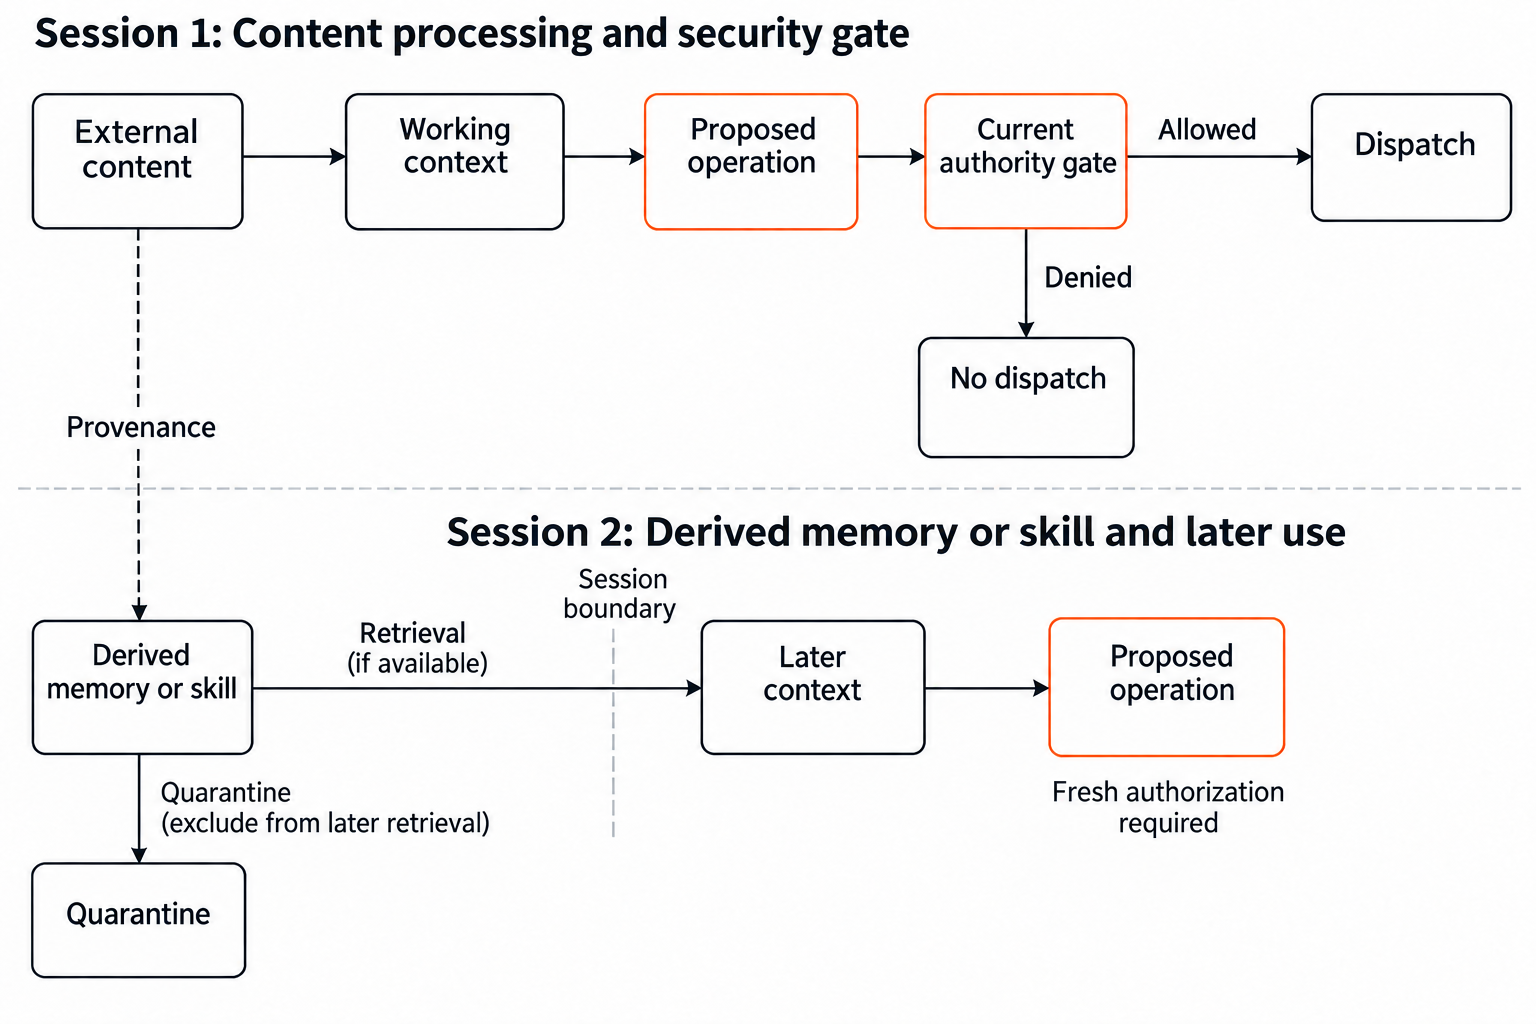
\includegraphics[width=\linewidth]{book/figures/assets/F28review.png}
\caption{Untrusted content can persist through derived memory or skills after the original input disappears. Application-controlled quarantine excludes a retained record from later retrieval; current authorization constrains dispatch. The first-session decision does not authorize a later operation: fresh authorization is required before its dispatch, which is not depicted. An allowed operation may still be factually wrong, and these controls do not undo committed effects.}
\label{fig:C28:overview}
\end{figure}
